%%%%%%%%%%%%%%%%%%%%%%%%%%%%%%%%%%%%%%%%%%%%%%%%%%%%%%%%%%%%%%%%%%%%%%
% Edit the title below to update the display in My Documents
%\title{Project Report}
%
%%% Preamble
\documentclass[paper=a4, fontsize=11pt]{scrartcl}
\usepackage[T1]{fontenc}
\usepackage{fourier}

\usepackage[english]{babel}															% English language/hyphenation
\usepackage[protrusion=true,expansion=true]{microtype}	
\usepackage{amsmath,amsfonts,amsthm} % Math packages
\usepackage[pdftex]{graphicx}	
\usepackage{url}
\usepackage{color}
\usepackage{graphicx}
\usepackage[dvipsnames]{xcolor}
\usepackage{subfig}
\usepackage{float}



%%% Custom sectioning
\usepackage{sectsty}
\allsectionsfont{\centering \normalfont\scshape}


%%% Custom headers/footers (fancyhdr package)
\usepackage{fancyhdr}
\pagestyle{fancyplain}
\fancyhead{}											% No page header
\fancyfoot[L]{}											% Empty 
\fancyfoot[C]{}											% Empty
\fancyfoot[R]{\thepage}									% Pagenumbering
\renewcommand{\headrulewidth}{0pt}			% Remove header underlines
\renewcommand{\footrulewidth}{0pt}				% Remove footer underlines
\setlength{\headheight}{13.6pt}

%%% Insert hyperlinks
\usepackage{hyperref} 

%%% Equation and float numbering
\numberwithin{equation}{section}		% Equationnumbering: section.eq#
\numberwithin{figure}{section}			% Figurenumbering: section.fig#
\numberwithin{table}{section}				% Tablenumbering: section.tab#


%%% Maketitle metadata
\newcommand{\horrule}[1]{\rule{\linewidth}{#1}} 	% Horizontal rule

\title{
		%\vspace{-1in} 	
		\usefont{OT1}{bch}{b}{n}
		\normalfont \normalsize \textsc{IITM-CS4011 : Principles of Machine Learning} \\ [25pt]
		\horrule{0.5pt} \\[0.4cm]
		\huge Programming Assignment 2 \\
		\horrule{2pt} \\[0.5cm]
}
\author{
		\normalfont 								\normalsize
        EE15B025 : Ganga Meghanath\\[-3pt]		\normalsize
        \today
}
\date{}


%%% Begin document
\begin{document}
\maketitle
\section*{Feature Extraction}
\subsection{Principal Component Analysis : (PCA)}
PCA is mathematically defined as an orthogonal linear transformation that transforms the data to a new coordinate system.It can be thought of as fitting an n-dimensional ellipsoid to the data, where each axis of the ellipsoid represents a principal component. If some axis of the ellipsoid is small, then the variance along that axis is also small, and by omitting that axis and its corresponding principal component from our representation of the dataset, we lose only a small amount of information.\\\\

A 3-dimensional dataset (DS3) has been provided. It contains two classes. Principal Component Analysis (PCA) is performed on this dataset and a single feature is extracted. The data in this projected space is used to train Linear Regression with indicator random variables. The learnt model has been used for classifying the test instances. \\\\
The results obtained are shown below :\\

\begin{table}[H]
\label{T:equipos}
\begin{center}
\begin{tabular}{| c | c | c | c |}
\hline
\textbf{Labels} & \multicolumn{3}{ c |}{\textbf{Per Class Estimates}}  \\ 
\cline{2-4}
& \textbf{Precision} & \textbf{Recall} & \textbf{F-measure} \\
\hline

Class 1 & 0.611940298507  & 0.615 & 0.613466334165  \\ \hline
Class 2 & 0.613065326633 & 0.61 & 0.611528822055 \\ \hline
Overall Accuracy & \multicolumn{3}{c |}{61.25 $\%$} \\ \cline{2-4} \hline

\end{tabular}
\end{center}
\end{table}

\graphicspath{ {../EE15B025_PA2/Code/q1/} }
\begin{figure}[H]
  \centering
  \subfloat{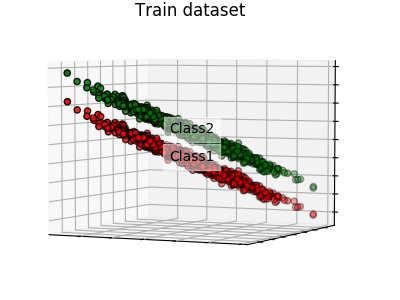
\includegraphics[width=0.5\textwidth]{q1_1}\label{fig:f1}}
  \hfill
  \subfloat{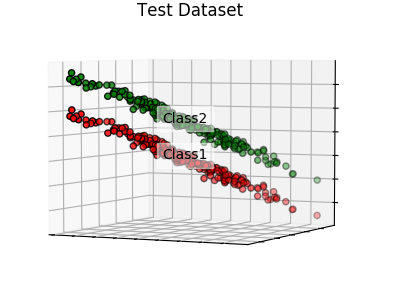
\includegraphics[width=0.5\textwidth]{q1_3}\label{fig:f2}}
  \caption*{The 3D plot of the Dataset}
\end{figure}

\begin{figure}[H]
  \centering
  \subfloat{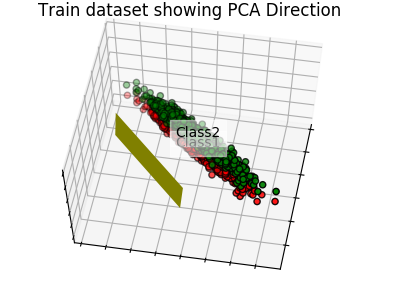
\includegraphics[width=0.5\textwidth]{q1_2}\label{fig:f1}}
  \hfill
  \subfloat{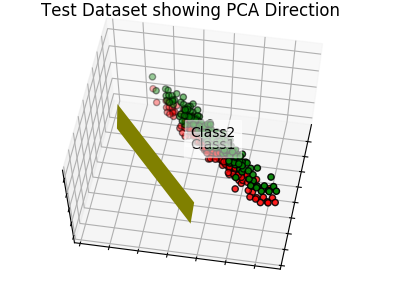
\includegraphics[width=0.5\textwidth]{q1_4}\label{fig:f2}}
  \caption*{The 3D plot of the Dataset with PCA Direction}
\end{figure}

\begin{center}
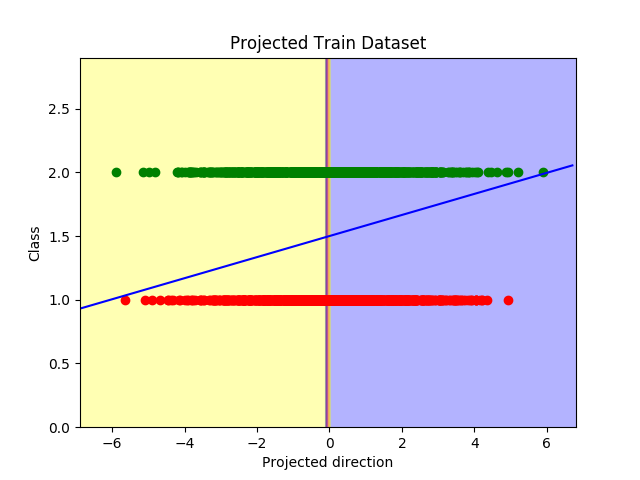
\includegraphics[scale=0.5]{q1_5}
\end{center}

\begin{center}
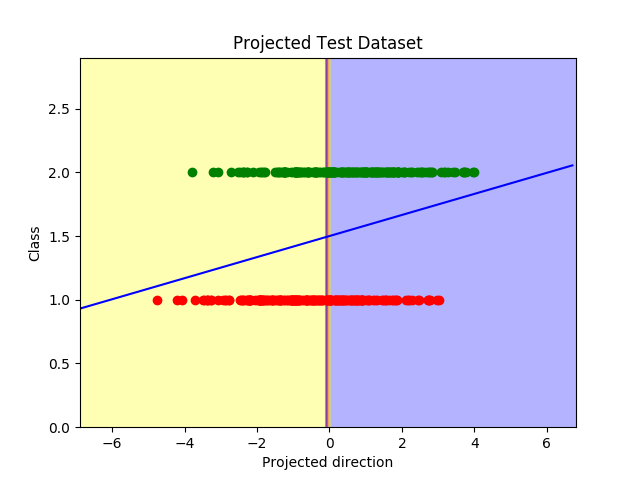
\includegraphics[scale=0.5]{q1_6}
\end{center}

The dataset depicted on the projected space along with the classifier boundary (y-axis:class)\\

The brown line indicates the decision boundary and the blue line indicates the predictions obtained from linear regression along the x-axis.

\subsection{Linear Discriminant Analysis : (LDA)}
Linear Discriminant Analysis is most commonly used as dimensionality reduction technique in the pre-processing step for machine learning applications. The goal is to project a dataset onto a lower-dimensional space with good class-separability in order avoid overfitting and also reduce computational costs.\\\\
A 3-dimensional dataset (DS3) has been provided. It contains two classes. Linear Discriminant Analysis (LDA) is performed on this dataset and a single feature is extracted. The data in this projected space is used to train Linear Regression with indicator random variables. The learnt model has been used for classifying the test instances. \\\\The results obtained are shown below :\\

\begin{table}[H]
\label{T:equipos}
\begin{center}
\begin{tabular}{| c | c | c | c |}
\hline
\textbf{Labels} & \multicolumn{3}{ c |}{\textbf{Per Class Estimates}}  \\ 
\cline{2-4}
& \textbf{Precision} & \textbf{Recall} & \textbf{F-measure} \\
\hline

Class 1 & 1.0 & 1.0 & 1.0 \\ \hline
Class 2 & 1.0 & 1.0  & 1.0 \\ \hline
Overall Accuracy & \multicolumn{3}{c |}{100 $\%$} \\ \cline{2-4} \hline

\end{tabular}
\end{center}
\end{table}

\graphicspath{ {../EE15B025_PA2/Code/q2/} }
\begin{figure}[H]
  \centering
  \subfloat{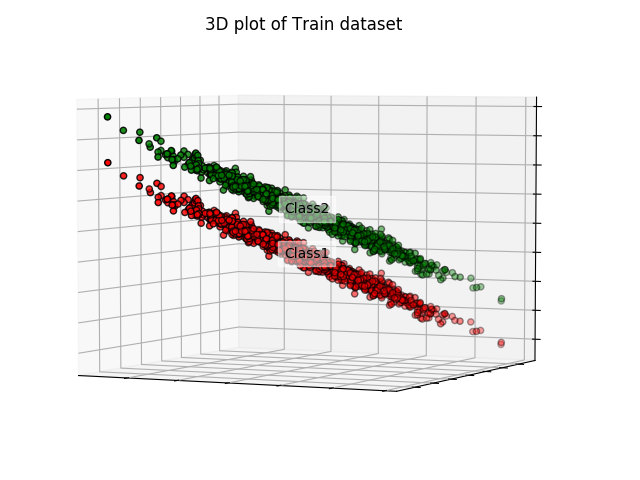
\includegraphics[width=0.5\textwidth]{q2_1}\label{fig:f1}}
  \hfill
  \subfloat{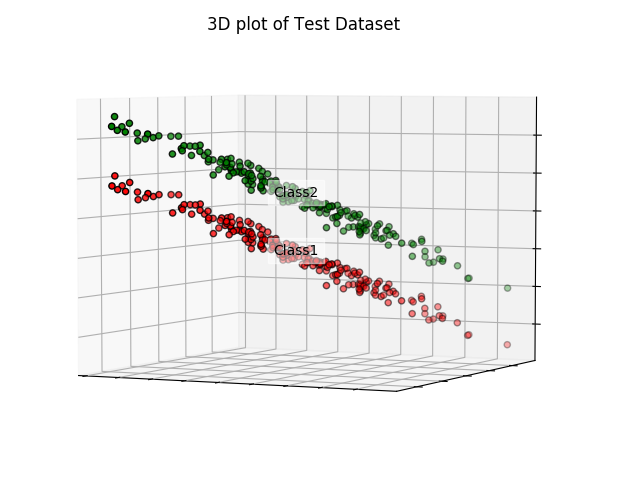
\includegraphics[width=0.5\textwidth]{q2_3}\label{fig:f2}}
  \caption*{The 3D plot of the Dataset}
\end{figure}

\begin{figure}[H]
  \centering
  \subfloat{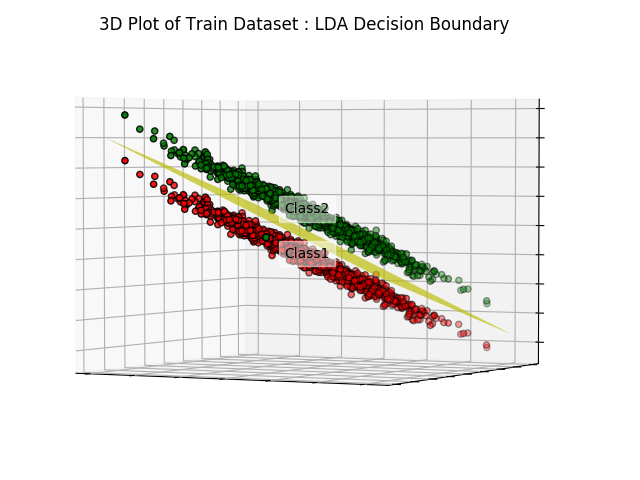
\includegraphics[width=0.5\textwidth]{q2_2}\label{fig:f1}}
  \hfill
  \subfloat{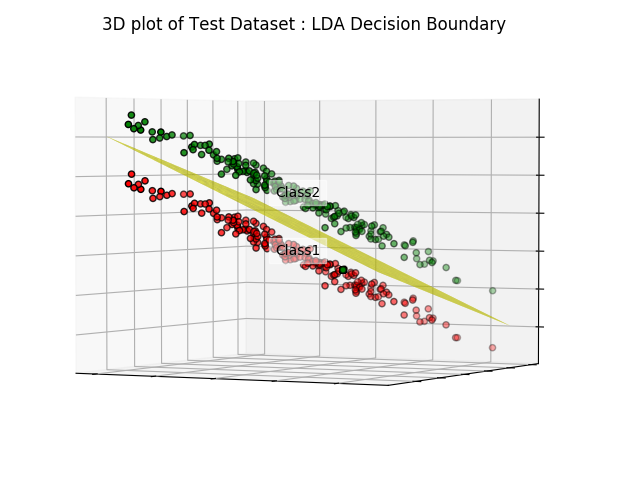
\includegraphics[width=0.5\textwidth]{q2_4}\label{fig:f2}}
  \caption*{The 3D plot of the Dataset with PCA Direction}
\end{figure}

\begin{center}
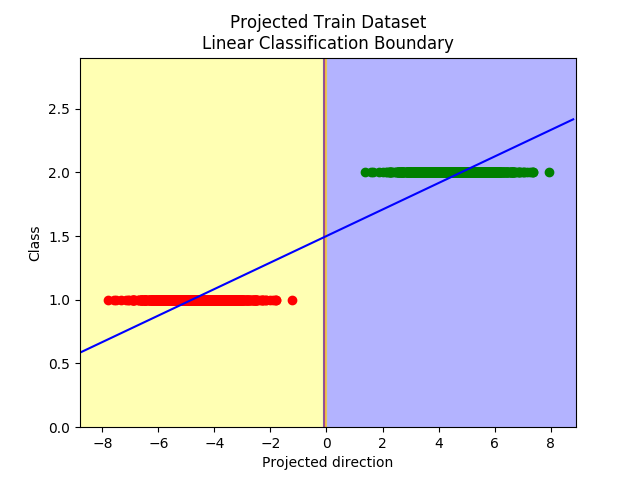
\includegraphics[scale=0.5]{q2_5}
\end{center}

\begin{center}
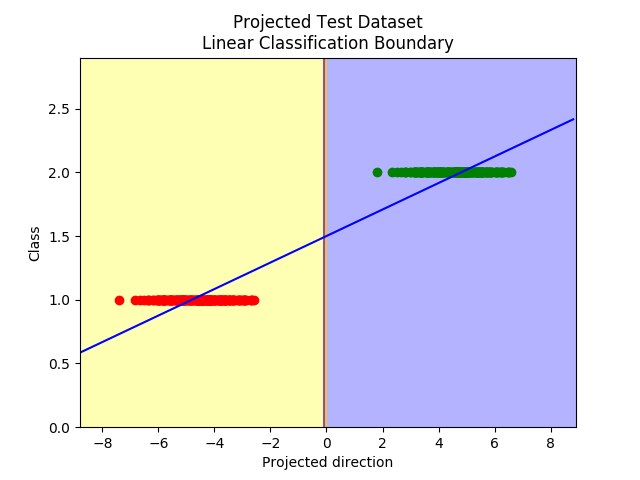
\includegraphics[scale=0.5]{q2_6}
\end{center}

The dataset depicted on the projected space along with the classifier boundary (y-axis:class)\\

The brown line indicates the decision boundary and the blue line indicates the predictions obtained from linear regression along the x-axis.


\subsection*{Comparison between PCA and LDA}
As we can observe, LDA gives better results on the same dataset as compared to PCA when it comes to classification. This is because, in the case of a single derived feature, PCA attempts to find the direction in which overall variance of the dataset is maximum and the dataset is projected onto this direction, whereas in the case of LDA, it tries to find a direction that maximises the ratio of 'between class variance' and 'within class variance'. Hence, LDA tries to maximise the variance (or distance) between the two classes, while minimising the variance within a class, which is exactly what we want for classification purposes. Essentially, LDA explicitly attempts to model the difference between the classes of data, whereas PCA on the other hand does not take into account any difference in class. As a result, LDA gives better features for classification as compared to PCA.

\subsection{LDA and its variants : QDA and RDA}
Quadratic discriminant analysis (QDA) is closely related to linear discriminant analysis (LDA), where it is assumed that the measurements from each class are normally distributed. Unlike LDA however, in QDA there is no assumption that the covariance of each of the classes is identical. Hence, the discriminant function is a quadratic function and will contain second order terms.\\
Regularized discriminant analysis is sort of a trade-off between LDA and QDA. RDA shrinks the separate covariances of QDA toward a common covariance as in LDA. The parameter $\alpha$ (\textcolor{Brown}{reg$\_$param} in the QDA function in sklearn) controls the complexity of the model.In an extreme case, if $\alpha$ = 1, then the second term is zero and you get what you would with QDA. If $\alpha$ = 0, then you  get what you would with LDA.\\\\
\begin{equation*}
{\hat\Sigma}_{k}(\alpha) = \alpha{\hat\Sigma}_{k} + (1-\alpha){\Sigma_{k}}
\end{equation*}
${\hat\Sigma}_{k}(\alpha)$ is a convex combination of the common covariance matrix in LDA and a separate covariance matrix estimated as in QDA. (Note : sklearn regularizes the covariance estimate as (1-reg$\_$param)*Sigma + reg$\_$param*np.eye(n$\_$features))\\
The decision boundaries learned by LDA, QDA and RDA have been visualised for Iris Dataset from \textcolor{blue}{\url{http://archive.ics.uci.edu/ml/datasets/Iris/}}. (Only petal width and petal length features have been utilised as attributes) \\

The boundaries learnt after performing LDA and QDA are as follows :\\

\graphicspath{ {../EE15B025_PA2/Code/q3/} }
\begin{center}
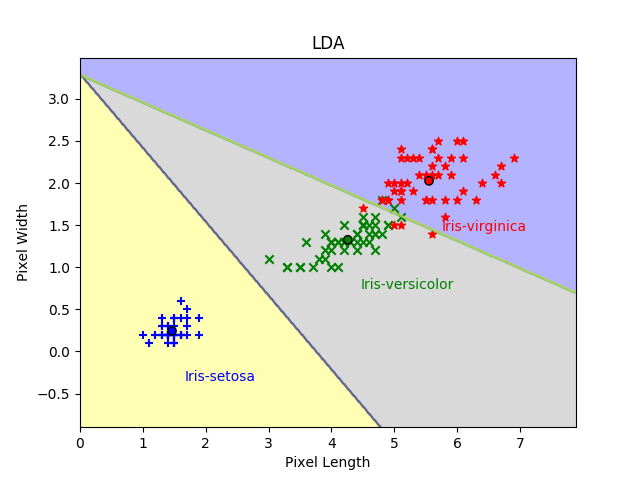
\includegraphics[scale=0.6]{LDA}
\end{center}

\begin{center}
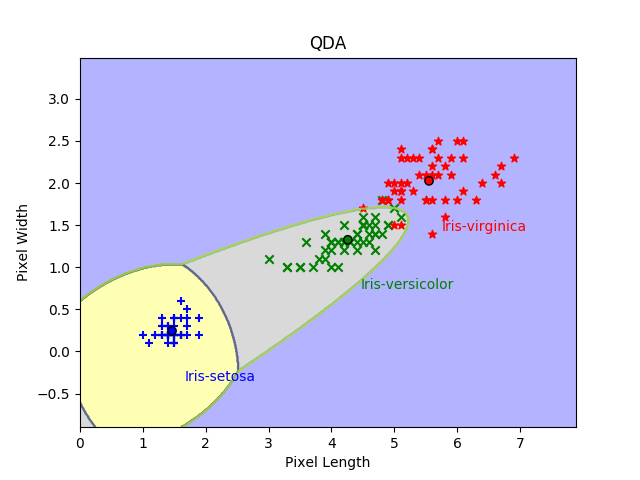
\includegraphics[scale=0.6]{QDA}
\end{center}
The boundaries learnt after performing RDA is as follows :\\

\begin{figure}[H]
  \centering
  \subfloat[$\alpha = 0.01$]{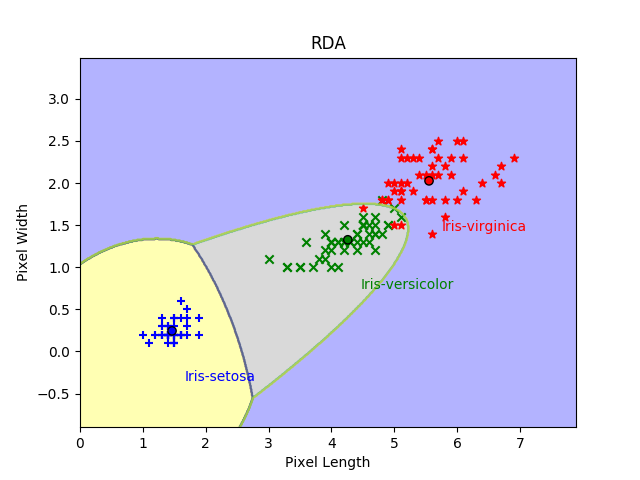
\includegraphics[width=0.5\textwidth]{001}}
  \hfill
  \subfloat[$\alpha = 0.05$]{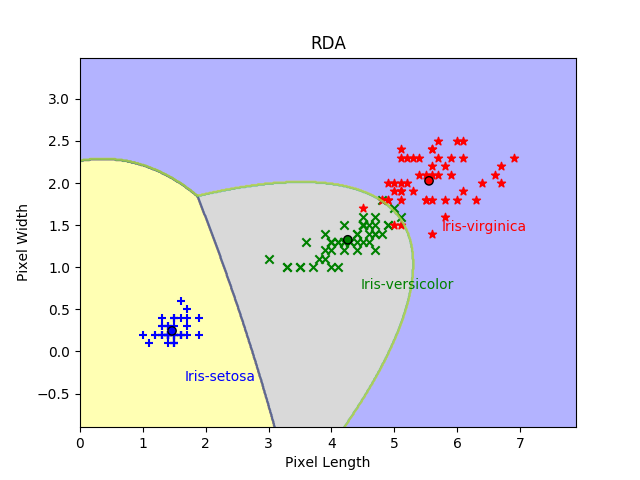
\includegraphics[width=0.5\textwidth]{005}}
  \vfill
  \subfloat[$\alpha = 0.1$]{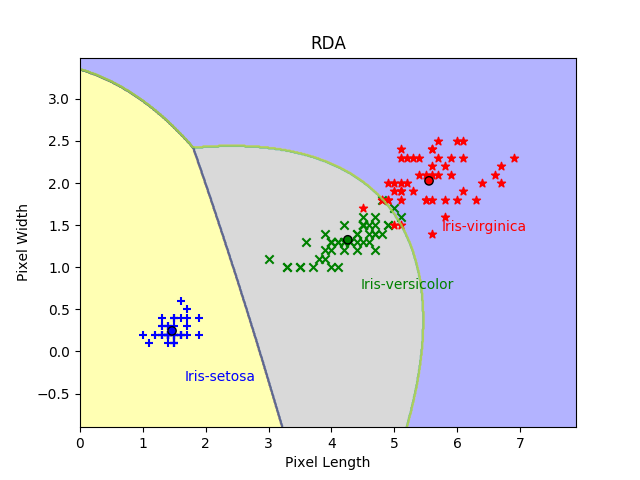
\includegraphics[width=0.5\textwidth]{01}}
  \hfill
  \subfloat[$\alpha = 0.25$]{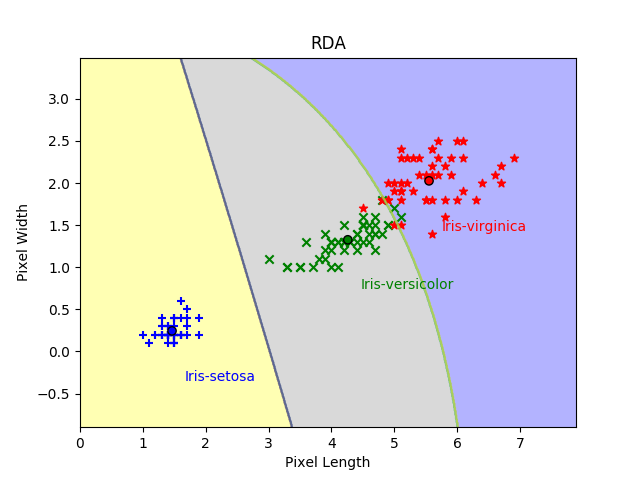
\includegraphics[width=0.5\textwidth]{0_25}}
  \vfill
  \subfloat[$\alpha = 0.5$]{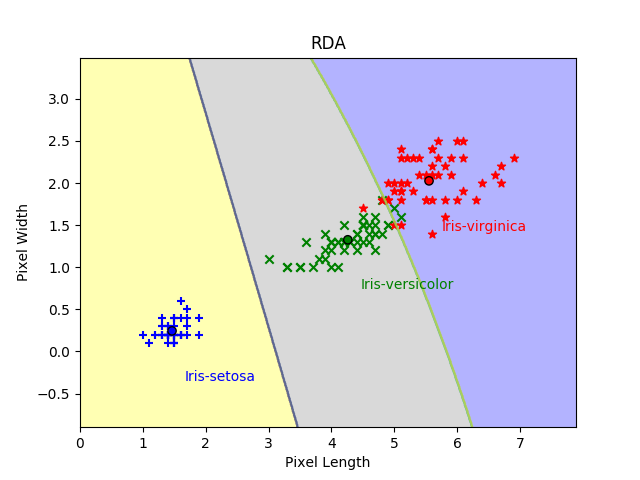
\includegraphics[width=0.5\textwidth]{05}}
  \hfill
  \subfloat[$\alpha = 0.75$]{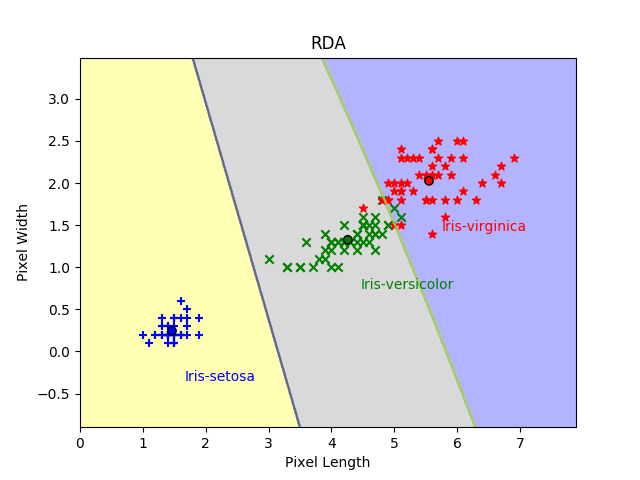
\includegraphics[width=0.5\textwidth]{0_75}}
\end{figure}

\section*{SVM}
Support Vector Machines (SVMs) are supervised learning models with associated learning algorithms that analyze data used for classification and regression. In addition to performing linear classification, SVMs can efficiently perform a non-linear classification using what is called the kernel trick, implicitly mapping their inputs into high-dimensional feature spaces.(Classification has been demonstrated below).\\
The dataset DS2 has been utilised for the classification. The objective is to train an SVM to classify the test images into either of the following four categories: 
\begin{center}
	{coast} \\
	{forest} \\
	{inside-city}\\ 
	{mountain}\\
\end{center}

The python sklearn package has functions that help implement libsvm with the concerned kernels. "\textcolor{Brown}{data$\_$creation.py}" converts the datasets to \textcolor{Brown}{libsvm format} as train and test.
\graphicspath{ {../EE15B025_PA2/Code/q4/} }
\begin{figure}[H]
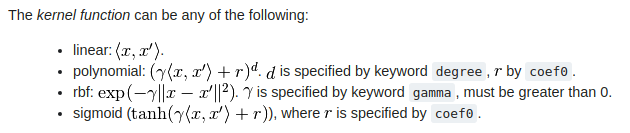
\includegraphics[scale=0.72]{kernel}
\end{figure}


\subsection*{Linear Kernel}
The model has been selected after analysing the average accuracy obtained on doing a cross-validation using 10 different batches. A Stratified K-Folds cross-validator has been used for the purpose of creating the batches. Different models were tested by varying the value of the penality 'C'. The best model obtained has been saved in 'svm$\_$model1.model' in the 'Models' folder. The best 3 results obtained are listed below :

\begin{table}[H]
\label{T:equipos}
\begin{center}
\begin{tabular}{| c | c |}
\hline
\textbf{C} & \textbf{Accuracy} \\
\hline

0.1 & 0.65 \\ \hline
4.71423423423 & 0.6 \\ \hline
5.27263157895 & 0.6 \\ \hline

\end{tabular}
\end{center}
\end{table}

The results for the best model is as follows :
\begin{table}[H]
\label{T:equipos}
\begin{center}
\begin{tabular}{| c | c | c | c |}
\hline
\textbf{Labels} & \multicolumn{3}{ c |}{\textbf{Per Class Estimates}}  \\ 
\cline{2-4}
& \textbf{Precision} & \textbf{Recall} & \textbf{F-measure} \\
\hline

coast &  0.59   &   0.50   &   0.54   \\ \hline
forest &  0.68   &   0.85   &   0.76  \\ \hline
inside-city &  0.60   &   0.60   &   0.60  \\ \hline
mountain &  0.72   &   0.65   &   0.68 \\ \hline

\end{tabular}
\end{center}
\end{table}

\subsection*{Polynomial Kernel}
The model has been selected after analysing the average accuracy obtained on doing a cross-validation using 10 different batches. A Stratified K-Folds cross-validator has been used for the purpose of creating the batches. Different models were tested by varying the value of the penality 'C', degree of the polynomial 'd', Kernel coefficient '$\gamma$' and the independent term 'coef0'. The best model obtained has been saved in 'svm$\_$model2.model' in the 'Models' folder. The best 3 results obtained are listed below :

\begin{table}[H]
\label{T:equipos}
\begin{center}
\begin{tabular}{| c | c | c | c | c |}
\hline
\textbf{Degree} & \textbf{C} & \textbf{$\gamma$} & \textbf{Coef0} & \textbf{Accuracy} \\
\hline

2 & 0.0164285714286 & 8.0 & 2.14285714286 & 0.65306122449 \\ \hline
2 & 3.8125 & 0.5125 & 0.0 & 0.591836734694 \\ \hline
2 & 0.1 & 0.1 & 3.0 & 0.510204081633\\ \hline

\end{tabular}
\end{center}
\end{table}

The results for the best model is as follows :
\begin{table}[H]
\label{T:equipos}
\begin{center}
\begin{tabular}{| c | c | c | c |}
\hline
\textbf{Labels} & \multicolumn{3}{ c |}{\textbf{Per Class Estimates}}  \\ 
\cline{2-4}
& \textbf{Precision} & \textbf{Recall} & \textbf{F-measure} \\
\hline

coast & 0.64    &  0.35    &  0.45  \\ \hline
forest &  0.80   &   0.80   &   0.80 \\ \hline
inside-city &  0.55   &   0.80    &  0.65  \\ \hline
mountain &   0.45   &   0.45    &  0.45  \\ \hline

\end{tabular}
\end{center}
\end{table}

\subsection*{Gaussean Kernel}
The model has been selected after analysing the average accuracy obtained on doing a cross-validation using 10 different batches. A Stratified K-Folds cross-validator has been used for the purpose of creating the batches. Different models were tested by varying the value of the penality 'C' and the Kernel coefficient '$\gamma$'. The best model obtained has been saved in 'svm$\_$model3.model' in the 'Models' folder. The best result obtained using the chosen model is listed below :

\begin{table}[H]
\label{T:equipos}
\begin{center}
\begin{tabular}{| c | c | c |}
\hline
\textbf{C} & \textbf{$\gamma$} & \textbf{Accuracy} \\
\hline

94.7373684211 & 0.01 & 0.6625\\ \hline
3.31081081081 & 0.501351351351 & 0.6375\\ \hline
10.0 & 0.21387755102 & 0.6375\\ \hline

\end{tabular}
\end{center}
\end{table}

The results for the best model is as follows :
\begin{table}[H]
\label{T:equipos}
\begin{center}
\begin{tabular}{| c | c | c | c |}
\hline
\textbf{Labels} & \multicolumn{3}{ c |}{\textbf{Per Class Estimates}}  \\ 
\cline{2-4}
& \textbf{Precision} & \textbf{Recall} & \textbf{F-measure} \\
\hline

coast &   0.56   &   0.45   &   0.50    \\ \hline
forest &  0.84   &  0.80    &  0.82  \\ \hline
inside-city &  0.64   &   0.90   &   0.75  \\ \hline
mountain &  0.59   &   0.50   &   0.54   \\ \hline

\end{tabular}
\end{center}
\end{table}

\subsection*{Sigmoid Kernel}
The model has been selected after analysing the average accuracy obtained on doing a cross-validation using 10 different batches. A Stratified K-Folds cross-validator has been used for the purpose of creating the batches. Different models were tested by varying the value of the penality 'C', Kernel coefficient '$\gamma$' and the independent term 'coef0'. The best model obtained has been saved in 'svm$\_$model4.model' in the 'Models' folder. The best result obtained using the chosen model is listed below :

\begin{table}[H]
\label{T:equipos}
\begin{center}
\begin{tabular}{| c | c | c | c |}
\hline
\textbf{C} & \textbf{$\gamma$} & \textbf{Coef0} & \textbf{Accuracy} \\
\hline

500.0 & 0.0111020408163 & 0.0 & 0.755102040816\\ \hline
212.040816327 & 0.021387755102 & 0.0 & 0.734693877551\\ \hline
73.6868421053 & 0.01 & 0.01 & 0.612244897959\\ \hline	

\end{tabular}
\end{center}
\end{table}

The results for the best model is as follows :

\begin{table}[H]
\label{T:equipos}
\begin{center}
\begin{tabular}{| c | c | c | c |}
\hline
\textbf{Labels} & \multicolumn{3}{ c |}{\textbf{Per Class Estimates}}  \\ 
\cline{2-4}
& \textbf{Precision} & \textbf{Recall} & \textbf{F-measure} \\
\hline

coast &   0.59   &   0.50   &   0.54   \\ \hline
forest &   0.71   &   0.60   &   0.65   \\ \hline
inside-city &  0.59   &   0.80  &    0.68  \\ \hline
mountain &     0.58    &  0.55  &    0.56    \\ \hline

\end{tabular}
\end{center}
\end{table}

Hence, the best accuracy was achieved using a sigmoidal kernel in the various trials conducted using the given dataset and different c-SVM parameters.

\section*{Decision Trees}
The entire problem has been done using Weka. Mushroom dataset (2-class problem with 8124 instances) from UCI machine learning repository \textcolor{blue}{\url{https://archive.ics.uci.edu/ml/datasets/Mushroom}} has been used. The last 1124 instances are used as test data and the rest as training data.\\

The python file '\textcolor{Brown}{Dataset$\_$creation.py}' reads the dataset, segregates it as training and testing data with 7000 and 1124 instances each and converts them into the format ARFF and creates the training and testing files 'mushroom$\_$train.arff' and 'mushroom$\_$test.arff'. \\

The models obtained by the decision trees have been saved in the folder '\textcolor{Brown}{Models}'. The format used is 'cross$\_$valid$\_$<MinNumObj>$\_$rp.model' and 'cross$\_$valid$\_$<MinNumObj>.model'. 'rp' signifies that Reduced Error Pruning has been done on the tree. \\

The trees obtained using the models have been saved in the folder '\textcolor{Brown}{Trees}'. The format used is 'cross$\_$valid$\_$<MinNumObj>$\_$rp.png' and 'cross$\_$valid$\_$<MinNumObj>.png'. 'rp' signifies that Reduced Error Pruning has been done on the tree. \\

The results obtained using the models have been saved in the folder '\textcolor{Brown}{Results}'. The format used is 'cross$\_$valid$\_$<MinNumObj>$\_$rp' and 'cross$\_$valid$\_$<MinNumObj>'. 'rp' signifies that Reduced Error Pruning has been done on the tree. \\

MinNumObj refers to the minimum number of datapoints in each leaf. We can observe from the table that, as the MinNumObj value decreases, the tree becomes bigger and more accurate in prediction and performs better both on training and test sets, and as the MinNumObj is increased, the tree becomes smaller and the accuracy of prediction or overall performance decreases. This is because, in case of a small value of MinNumObj, the tree will grow until each leaf has only a small number of datapoints and hence, the classifier performs better \\

Reduced Error Pruning refers to removing a subtree at some internal node and making it a leaf and assigning to it, the most common class at that node, as long as the performance on the validation set remains the same or decreases. We can see that the performance on the test data more or less remains the same even after pruning the tree, though the performance on the training data decreases a little in comparison to the situation when there is no pruning.\\

The effect of MinNumObj and Reduced Error Pruning has been depicted below : \\
\begin{table}[H]
\label{T:equipos}
\begin{center}
\begin{tabular}{| c | c | c | c |}
\hline
\textbf{MinNumObj} & \textbf{Reduced Error Pruning} & \textbf{Accuracy on train$\_$set} & \textbf{Accuracy on test$\_$set} \\ 
\hline

1 & No  & 99.9857 $\%$ & 100 $\%$ \\ \hline
1 & Yes  & 99.9571 $\%$ & 100 $\%$ \\ \hline
2 & No  & 99.9857 $\%$ & 100 $\%$ \\ \hline
2 & Yes & 99.9571 $\%$ & 100 $\%$ \\ \hline
5 & No & 99.9857 $\%$ & 100 $\%$ \\ \hline
5 & Yes & 99.9 $\%$ & 100 $\%$ \\ \hline
10 & No & 99.9857 $\%$ & 100 $\%$ \\ \hline
10 & Yes & 99.9 $\%$ & 100 $\%$ \\ \hline
25 & No & 99.8714 $\%$ & 99.3772 $\%$ \\ \hline
25 & Yes & 99.4286 $\%$ & 99.3772 $\%$ \\ \hline
50 & No & 99.4143 $\%$ & 99.3772 $\%$ \\ \hline
50 & Yes & 98.8714 $\%$ & 99.3772 $\%$ \\ \hline
100 & No & 98.3857 $\%$ & 99.3772 $\%$ \\ \hline
100 & Yes & 98.3857 $\%$ & 99.3772 $\%$ \\ \hline 


\end{tabular}
\end{center}
\end{table}

As we can observe from the above table, the best model would have MinNumObj=2 and we don't prune the tree. The confusion matrix for the test set is as follows :\\
\begin{table}[H]
\label{T:equipos}
\begin{center}
\begin{tabular}{| c | c | c |}
\hline
\textbf{Classified as} & \textbf{Edible} & \textbf{Poisonous} \\ 
\hline

Edible & 464  & 0 \\ \hline
Poisonous & 0 & 660 \\ \hline

\end{tabular}
\end{center}
\end{table}

The results obtained are as follows :\\
\begin{table}[H]
\label{T:equipos}
\begin{center}
\begin{tabular}{| c | c | c | c |}
\hline
\textbf{Class} & \textbf{Recall} & \textbf{Precision} & \textbf{F-Measure}\\ 
\hline

Edible & 1  & 1 & 1 \\ \hline
Poisonous & 1 & 1 & 1 \\ \hline

\end{tabular}
\end{center}
\end{table}
As we can infer from the tree given above, the important features in deciding whether a mushroom is edible or not are \textcolor{OliveGreen}{Odor}, \textcolor{OliveGreen}{Stalk-shape}, \textcolor{OliveGreen}{Spore-print-color}, \textcolor{OliveGreen}{Grill-size}, \textcolor{OliveGreen}{Grill-spacing} and \textcolor{OliveGreen}{Population}.\\\\
The tree generated :\\

\begin{figure}[H]
\begin{center}
\graphicspath{ {../EE15B025_PA2/Code/q5/Trees/} }
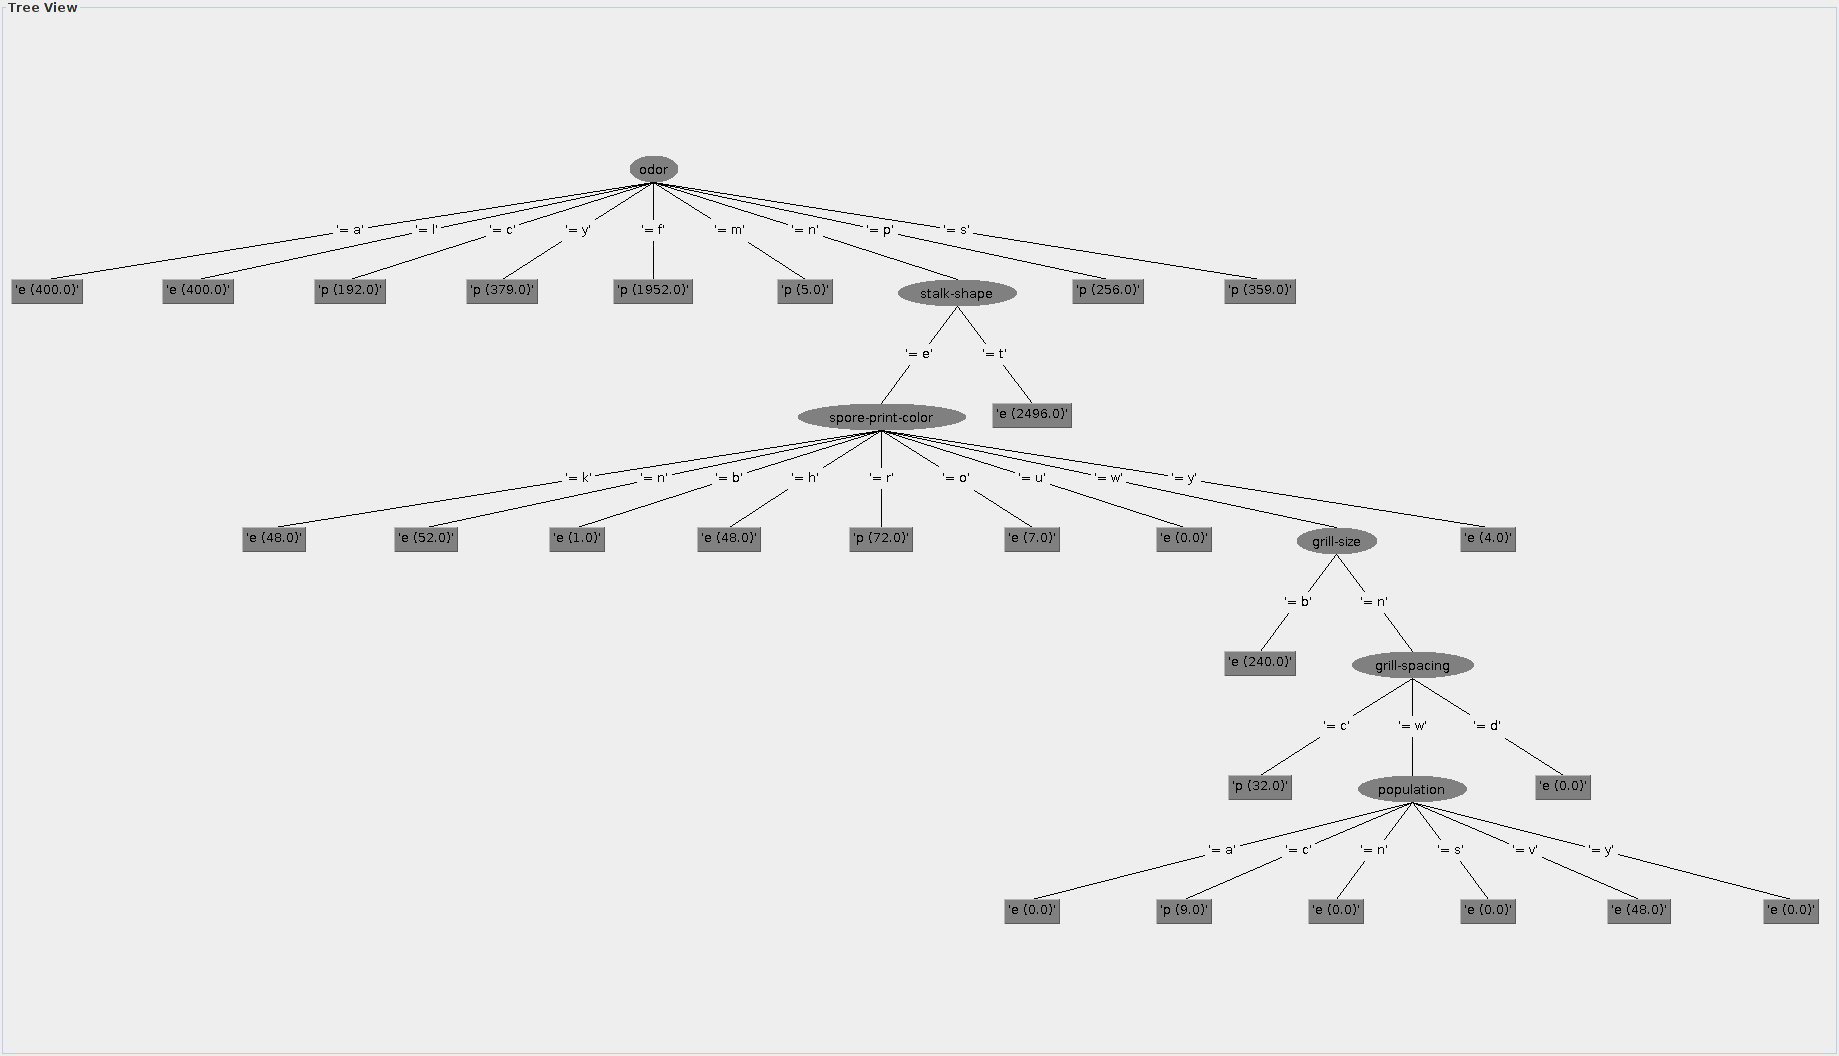
\includegraphics[scale=0.25]{cross_valid_2}
\end{center}
\end{figure}

With MinNumObj=100 and Reduced Error Pruning, we get 99.3772$\%$ accuracy on the test set and hence, the most important feature to decide whether a mushroom is edible or not is \textcolor{OliveGreen}{Odor} as we can see from the tree given below.

\begin{figure}[H]
\begin{center}
\graphicspath{ {../EE15B025_PA2/Code/q5/Trees/} }
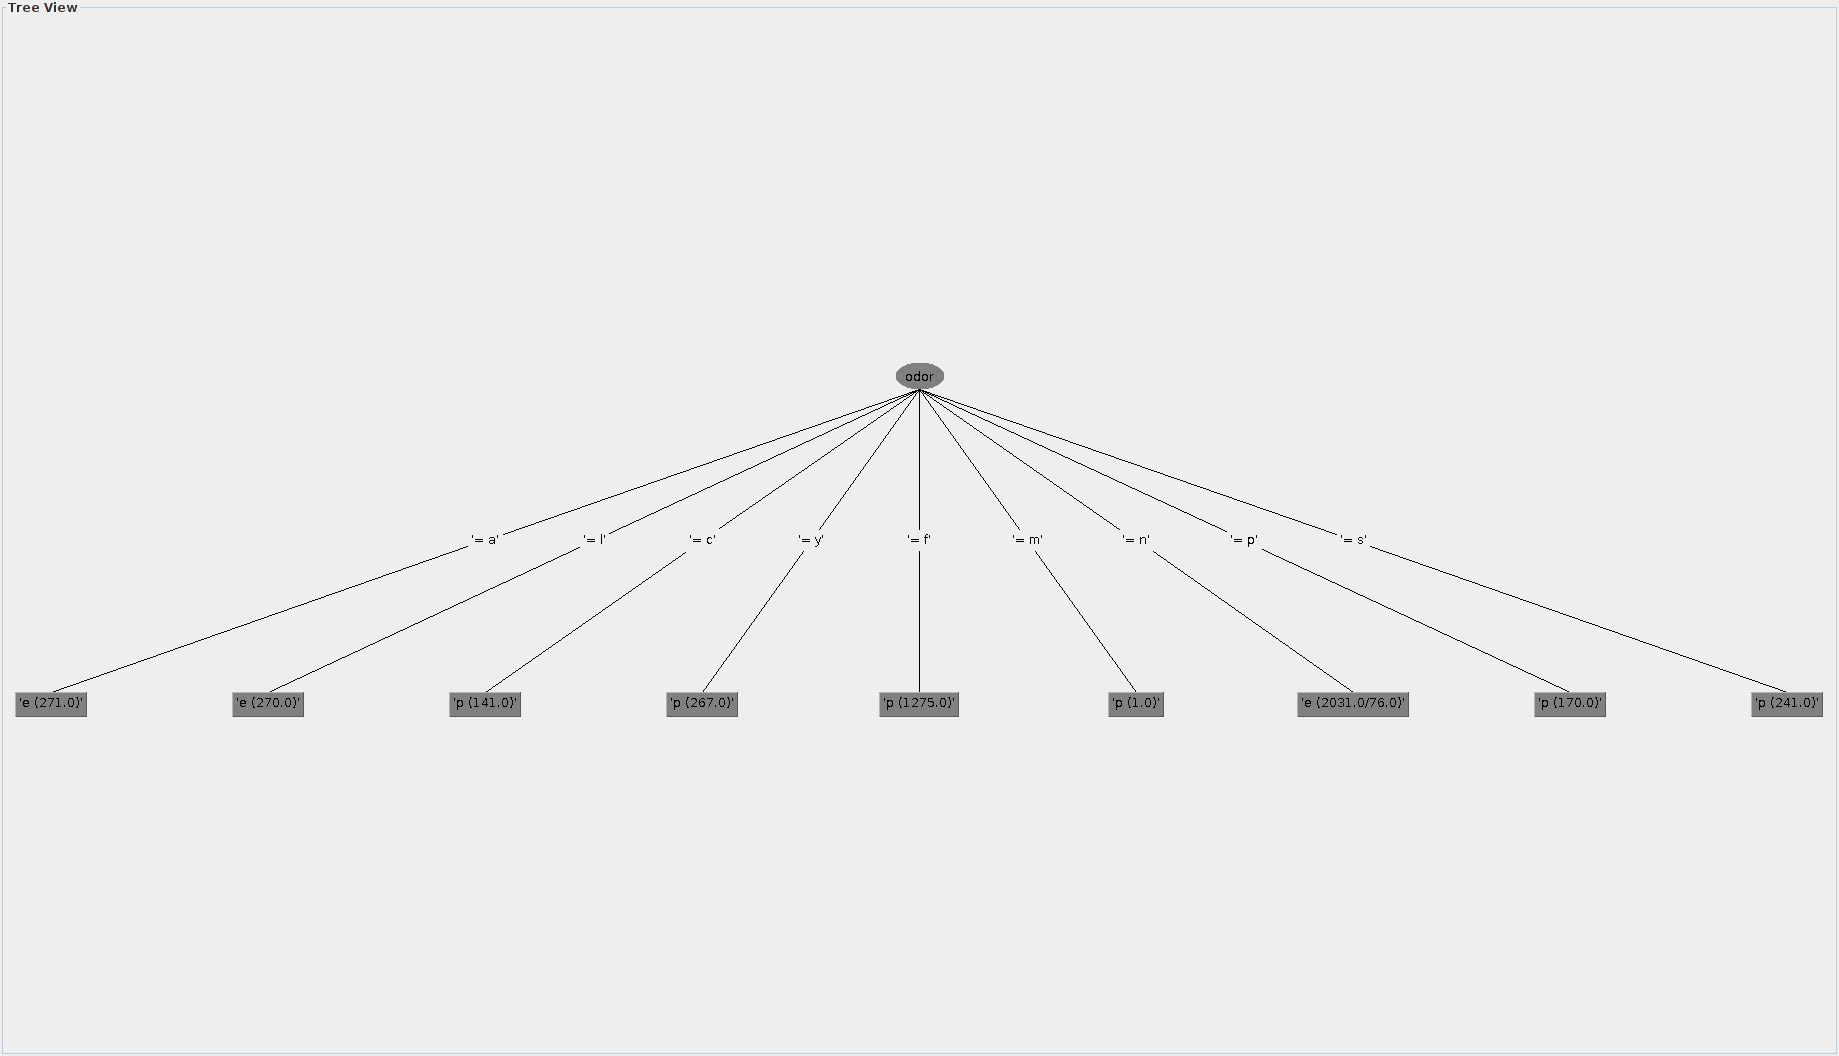
\includegraphics[scale=0.25]{cross_valid_100_rp}
\end{center}
\end{figure}

The confusion matrix for the test set is as follows :\\
\begin{table}[H]
\label{T:equipos}
\begin{center}
\begin{tabular}{| c | c | c |}
\hline
\textbf{Classified as} & \textbf{Edible} & \textbf{Poisonous} \\ 
\hline

Edible & 464  & 0 \\ \hline
Poisonous & 7 & 653 \\ \hline

\end{tabular}
\end{center}
\end{table}

The results obtained are as follows :\\
\begin{table}[H]
\label{T:equipos}
\begin{center}
\begin{tabular}{| c | c | c | c |}
\hline
\textbf{Class} & \textbf{Recall} & \textbf{Precision} & \textbf{F-Measure}\\ 
\hline

Edible & 1  & 0.985  & 0.993 \\ \hline
Poisonous & 0.989  & 1 & 0.995 \\ \hline

\end{tabular}
\end{center}
\end{table}

\end{document}